Focusing on the kind of recommendation system that we want to propose, we want to analyze what are the key features that our approach should support and what are the threats to face in this domain


\subsection{Opportunities}
From a general point of view, a recommendation system must provide a suggestion that must be complete, clear and easily integrable in the developer's context. Considering the code search engine, these features must be applied to the recommended snippet of code in order to improve the quality of the suggestion. A design choice that affects a code search engine is how it makes the query to get the results. From the literature, we see that there are two main technique: the interface-driven query, in which the user made by hand the query, and the keyword-based query, in which the tool uses directly the user's source code in order to retrieve the recommendations. Another key element in the design process of the application is the similarity criteria, that is the crucial part of this kind of system. There are a lot of techniques, that involves structural similarity, textual one, and fingerprints as well as semantic analysis of the code and conceptual metric, to measure the user's intentions beyond the source code. Regarding the implementation techniques, in recent years information retrieval and machine learning are the most common and rapidly growing in practice. In particular, most of the approaches use Lucene library to index the code and recover the needed information in very few time. Regarding machine learning techniques, neural networks and deep learning are common techniques to handle a big amount of data and face the classification problem. 

\subsection{Challenges}
So, considering all these possible manners to implement a recommendation system based on source code retrieval,  the main challenge is to choose the correct way to reach an excellent level of accuracy and precision to guarantee a useful hint for the developer. As we said, the key point is the similarity metric, that could bring bias if it is not properly defined, like false positive. Another point is the query building, that affects dramatically the results if is not well fixed. Of course, there are elements of uncertainty, like the user's behavior (in the interface-driven model) and the context (in the keyword-based model), that are not so easy to detect and prevent. Finally, we must consider also the time computation because the user wants the requested hint as soon as possible and she sees a delay as a severe issue. 

\subsection{Use case study}
To better understand the context in which we are, we provide a concrete example of a recommendation based on snippets of code.The typical setting considered in the paper is as shown in Fig.~\ref{fig:codeExample}:~a developer is implementing some method to 
satisfy the requirements of the system being developed. In the specific case 
shown in Fig.~\ref{fig:codeExample}.b, the \code{publish} method connects to an MQTT (Message Queuing Telemetry Transport) client and exposes a message over a channel by using the object 
\code{MqttMessage}. To this end, the \code{Eclipse Paho} 
library\footnote{\url{https://github.com/andypiper/paho-mqtt/blob/master/org.eclipse.paho.sample.mqttv3app/src/org/eclipse/paho/sample/mqttv3app/Sample.java}}
is used as it provides useful interfaces and classes to send and receive messages over the MQTT protocol.

\begin{figure}[h!]
	\centering
	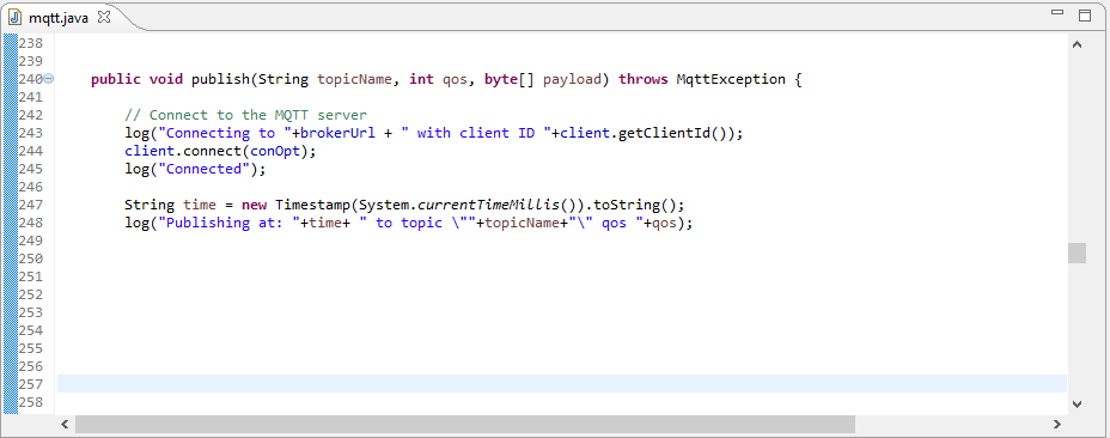
\includegraphics[width=\columnwidth]{figs/API-example} \\
	\scriptsize{a) Initial version} \\
	\vspace{.2cm}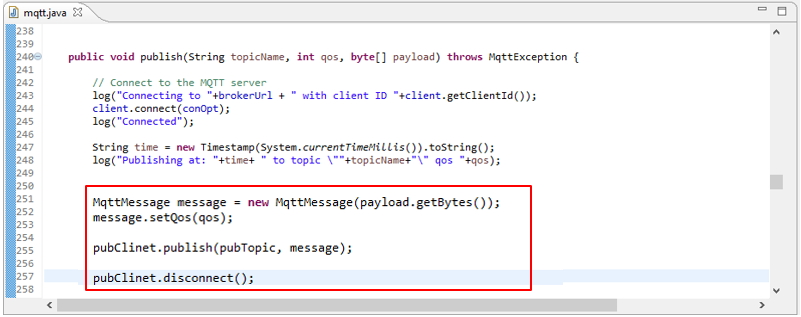
\includegraphics[width=\columnwidth]{figs/API-example-final} \\
	\scriptsize{b) Final version}\\
	\vspace{-.2cm}
	\caption{Use case study}
	\label{fig:codeExample}
\end{figure}

Fig.~\ref{fig:codeExample}.a depicts the situation where the development 
is at an early stage and the developer already used some methods of the chosen 
API to develop the required functionality. However, she is not sure how to 
proceed from this point. In such cases, different sources of information 
may be consulted, such as StackOverflow, video tutorials, API 
documentation, \etc. In this paper, we propose an approach aiming at providing 
developers with recommendations consisting of a list of API method 
calls that should be used next, and with usage patterns that can be used as a 
reference for completing the development of the method being defined (\eg code 
snippets that could support developers to complete the method definition with 
the framed code in Fig. \ref{fig:codeExample}.b).
